
% ------------------------------------------------------------------------------------------------------------------------------------------------
\chapter{System design}
\label{chap:system-design}

The system, from here to be referred to by the name ''\textit{Oculus}'', is designed with an asynchronous as well as distributed aproach in mind. In order to achieve high asynchrononisity between obtaining new reference data, and running jobs such as ''\textit{compare video1 with the reference database}'', the system was split into two primary components: 

\begin{itemize}
  \item \textbf{loader} -- which is responsible for obtaining more and more reference material. It persists and initially processes the videos, as well as any related metadata. In a real system this reference data would be provided by partnering content providers, yet for this 
  \item \textbf{analyser} -- which is responsible for preparing and scheduling job pipelines for execution on top of the Hadoop cluster and reference databases.
\end{itemize}

To further illustrate the separate components and their interactions Figure \ref{fig:system-overview} shows the different interactions within the system.

\begin{figure}[hc!]
 \centering
  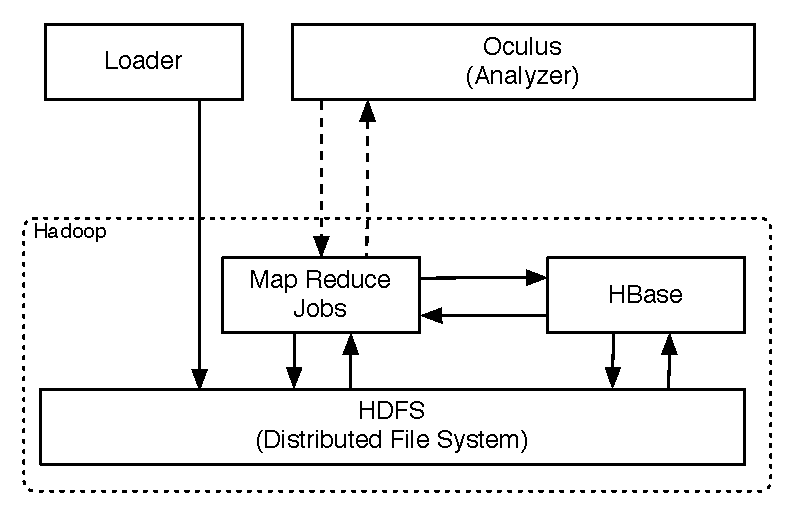
\includegraphics[scale=0.9]{./diagrams/high-level-system.pdf}
  \caption{High level overview of the system's architecture}
  \label{fig:system-overview}
\end{figure}

% ------------------------------------------------------------------------------------------------------------------------------------------------
\section{Loader}
\label{sec:loader-basics}
The Loader component is responsible for obtaining as much as possible ''reference data'', by which I mean video material -- from sites such as \textit{youtube.com} or video hosting sites. Please note that for the sake of this thesis (and legal safety) the downloaded content was limited to movie trailers (which are freely available on-line) as well as series opening, ending sequences.

While I will refer to the Loader (as a system) in singular, it should be noted that in fact there are multiple instances of it running in the cluster.
Thanks to the use of Akka's \cite{akka-docs} Actor Model abstractions (and \textit{remoting} module \cite{akka-remoting}), in which the physical location of an Actor plays is of no importance -- meaning, that the receiving Actor does not have to be on the same host as the sending Actor.

\subsection{Types of Actors used in the system}
\label{sec:types-of-actors}

The system consists of 4 types of Actors each of which has multiple instances which are spread out on many nodes in the cluster.
Some tasks can only be sent to local Actors (any work requiring an already downloaded file), but messages related to crawling and initially downloading
the video material can be spread throughout the cluster. I will now briefly describe the different Actor roles that exist in the system and then explain the interactions between then on an example.

\begin{itemize}
  \item \textbf{YouTubeCrawlActor} -- is capable of fetching and YouTube websites and generate Messages triggering
                                    either further crawling of ''related video sites'' (\verb|Crawl(siteId: String)|) or downloading of the 
                                    currently accessed video (by sending a \verb|Download(movieId)| message),
    \subitem  \textbf{receives:}
      \subsubitem 1 -- \verb|Crawl(siteId: String)| message
    \subitem  \textbf{sends:}
      \subsubitem 0 or n -- \verb|Crawl(siteId: String)| - where n is the number of ''related video'' links found on the site. 
                                                           If crawling is turned off, no messages will be sent.

  \item \textbf{DownloadActor} -- is responsible for downloading the movie from youtube in it's original format (in the presence of many formats, 
                                the highest quality file will be downloaded). This Actor decides if a video is legal to download or not, because it also
                                obtains the movie's metadata -- only trailers and opening sequences of series are downloaded during for the sake of this 
                                thesis.
                                
  \item \textbf{ConversionActor} -- is responsible for converting the downloaded video material into raw frame data (bitmaps).
    \subitem  \textbf{receives:}
      \subsubitem \verb|Convert(localVideoFile: java.util.File)| -- This message must come from a local Actor, since the path refers to the local file system.
    \subitem  \textbf{sends:}
      \subsubitem \verb|Upload(framesDirectory: java.util.File)| -- when the finished converting to bitmaps, it will send and \verb|Upload| 
                                                                    message to one of the\verb|HDFSUploadActors|, pointing to the directory where the 
                                                                    output bitmaps have been written.
                                                                    
  \item \textbf{HDFSUploadActor} -- is responsible for optimally storing the sequence of bitmaps in Hadoop. This includes converting a series of 
                                  relatively small (around 2MB per frame) files into one Sequence File on HDFS. Sequence Files and the need for their use
                                  will be explained in detail in section \ref{sec:sequence-files}.
  \subitem \textbf{receives:}
    \subsubitem \verb|Upload(framesDirectory: java.util.File)| -- pointing to a local directory where the bitmap files have been stored.
                                                                 This message must come from a local actor, since the path refers to the local file system.
\end{itemize}

% -------------------------------------------------------------------------------------------------------------------------------------------------
\newpage
\subsection{Obtaining reference video material}
\label{sec:obtaining-reference-material}
In this subsection I will discuss the process of obtaining video material by the Loader subsystem, as well as explain which parts can be executed on different nodes of the cluster. The Figure \ref{fig:high-level-loader} should help in understanding the basic workflow.

\begin{figure}[ch!]
  \centering
  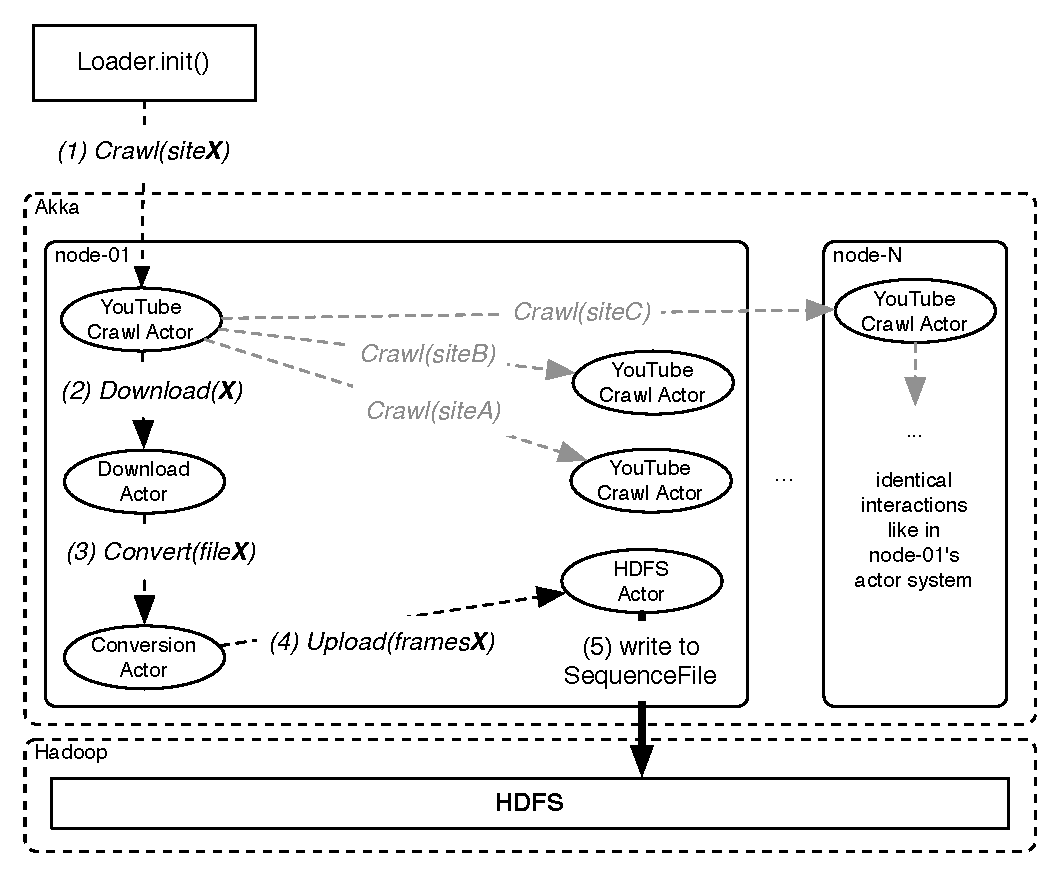
\includegraphics[scale=0.9]{./diagrams/loader-high-level.pdf}
  \caption{Overview of messages passed within the Loader's actor system. Greyed out messages are also sent, but are not on the critical path leading to obtaining material from \textit{siteX} into HDFS.}
  \label{fig:high-level-loader}
\end{figure}

\subsubsection{Step 1 - \textit{Crawl} messages}
The initiating message for each flow within the Loader is a \textit{Crawl(siteUrl)}, where siteUrl is a valid youtube video url.
The receiving YouTubeCrawlActor will react to such message by fetching and extracting the related video site urls and will forward those using the same kind of \textit{Crawl} messages. The second, yet most important, reaction is sending a \textit{Download(movieId)} message to an instance of an DownloadActor -- it  can reside on any node in the cluster, which allows us to spread the down-link utilisation between different nodes in the cluster.

It is worth pointing out that the receivers of these messages can be remote Actors, that is, can be located on a different node in the cluster than the sender. In order to guarantee spreading of the load among the many actors within the system (across nodes in the cluster), I am using a strategy called ''Smallest Inbox Routing''. This technique uses a special ''Router Actor'' which is responsible for a number of Routees (target Actors), and decides to deliver a message only to the Actor who has the smallest amount of messages ''not yet processed'' (which are kept in an Queue called the ''Inbox'', hence the strategy's name).

\subsubsection{Step 2 - \textit{Download} messages}
In the second step an \textit{YouTubeDownloadActor} instance receives a message asking it to download a movie.
It does so by invoking the native app \textit{youtube-dl}, which is an open source program specialised in downloading movies from YouTube.
Other than the video file (in an open source format) we also download a metadata description during this step, such metadata includes for example the date of publication, author, title and description of the movie. From this message including, all messages will be routed only to Actors local to the current node, because messages include \textit{File} objects, pointing to locations on-disk.

The metadata is then used to determine if it can be used in the context of this work, as only movie trailers and and opening / ending sequences are downloaded into the Oculus system. If the content is OK to use, the Actor sends an \textit{Convert(movieLocation)} message to an instance of \textit{ConversionActor}.

\subsubsection{Step 3 - \textit{Convert} messages}
The next step is executed by an instance of an \textit{ConversionActor} recieving an \textit{Convert(file)} message from another (local) Actor. The conversion phase will extract raw frame data from the incoming movie, and write those as plain bitmaps (not compressed) to files (one per each frame) into a specified target directory. The reason for not using a compressed lossless image format here is that all algorithms that the system will be dealing with later on are dealing with the raw image data, so we can avoid having to go over uncompression phases each time we will process a frame. Having that said, the storage format used for storing these files on HDFS provides build in compression (if enabeled), and it should be preferred in this case as it is transparent for the application, easing development of Map Reduce jobs in the Analyser system immensely.

The conversion from movie to raw bitmaps is performed by running an native application called \verb|ffmpeg| \cite{ffmpeg} instance (an de facto standard tool for such media operations), by forking a process from within the Actor. The CPU usage of running this extraction process easily reaches 100\% of the available resources, which is why the number of Conversion Actors per node is limited to only 1 per node, allowing ffmpeg to consume all available resources and finish extracting the data sooner. The actor will block until the process completes, and will then continue by sending an \textit{Upload(bitmapDirectory)} message to one of the \textit{HDFSUploadActors}.

\subsubsection{Step 4 \& 5 - \textit{Upload} messages}
The last step is an \textit{HDFSUploadActor} recieving an \textit{Upload(bitmapDirectory)} message which triggers it to connect to HDFS and start writing the bitmap data contained in the given directory to HDFS. The format of the generated data is as previously mentioned one file per frame of video, which averages around 2MB (depending on the movie resolution).

In this step the important part is that it does not write these files 1:1 onto HDFS, but instead writes into one file, using a hadoop specific storage format called ''Sequence File'', which allows for more efficient storage and latter retrieval of this data. Sequence Files, the need and benefits gained by using them as storage format for ''frame by frame'' data will be discussed in Section \ref{sec:sequence-files}.

This write terminates the operations performed on one movie by the Loader. All other operations will be performed by the Analyzer by running Map Reduce jobs on Sequence Files prepared in the above flow.

% ------------------------------------------------------------------------------------------------------------------------------------------------
\section{Analyser}
\label{sec:analyser}
The analyser component is responsible for orchestrating Map Reduce jobs and submitting them to the cluster. Results of jobs are written to either HBase or plain TSV (\textit{Tab Separated Values}) Files. Figure \ref{fig:analyser-high-level} depicts the typical execution flow of an analysis process issued by Oculus.

\begin{figure}[ch!]
  \centering
  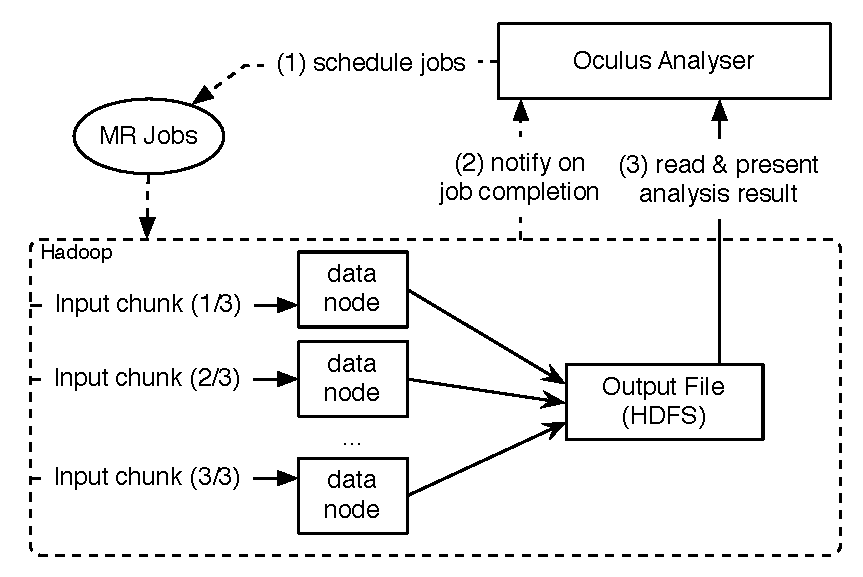
\includegraphics[scale=0.9]{diagrams/analyser-high-level.pdf}
  \caption{When storing a small file in HDFS, it still takes up an entire block. The grey space is not wasted on disk, but causes the \textit{name-node} memory problems.}
  \label{fig:analyser-high-level}
\end{figure}

In step 1 the \textit{job pipeline} is being prepared by the program by aggregating required metadata and preparing the job pipeline, which often consists of more than just one Map Reduce job -- in fact, most analysis jobs performed by Oculus require at least 3 or more Map Reduce jobs to be issued to the cluster. It is important to note that some of these jobs may be dependent on another task's output and this cannot be run in parallel. On the other hand, if a job requires calculating all histograms for all frames of a movie as well as calculating something different for each of these frames -- these jobs can be executed in parallel and will benefit from the large number of data nodes which can execute these jobs.

The 2nd step on Figure \ref{fig:analyser-high-level} is important because Oculus may react with launching another analysis job based on the notification that one pipeline has completed. This allows to keep different pipelines separate, and trigger them reactively when for example all it's dependencies have been computed in another pipeline.

For most applications though the 3rd step in a typical Oculus Job would be to read and present top N results to the issuer of the job, which for a question like ''Which movie is similar to this one?'' would be the top N most similar movies (their names, identifiers as well as match percentage).


% ------------------------------------------------------------------------------------------------------------------------------------------------
\subsection{Defining Map Reduce Pipelines using Scalding and Cascading}
TODO TODO THIS IS JUST SAMPLES
\todo{TODO TODO THIS IS JUST SAMPLES}

The primary language used for implementing all Oculus jobs, including Map Reduce jobs is Scala \cite{scala}

This is how an example job would look like:

\begin{lstlisting}[caption={Simplest Scalding job used in Oculus -- each frame perceptual hashing}, label={lst:simplest-scalding-job}]
  Tsv("input.tsv")
    .map('line -> 'word) { line: String => line.split }
    .groupBy('word) { _.count }
    .write(Tsv("output.tsv"))
\end{lstlisting}


\subsubsection{Parallel execution and job ordering}
Because a Scalding job (which effectively is an Cascading ''\textit{Pipeline}'') can span multiple Map Reduce Job invocations,
it is important to visualise how many actual Jobs will be submitted to the cluster and also if they can be run in parallel.

In order to visualise how jobs actually will be executed on the cluster Cascading provides a very important option allowing to print the resulting job
graph using the widely accepted graph-description language DOT \cite{dot}.

\begin{figure}[ch!]
  \centering
  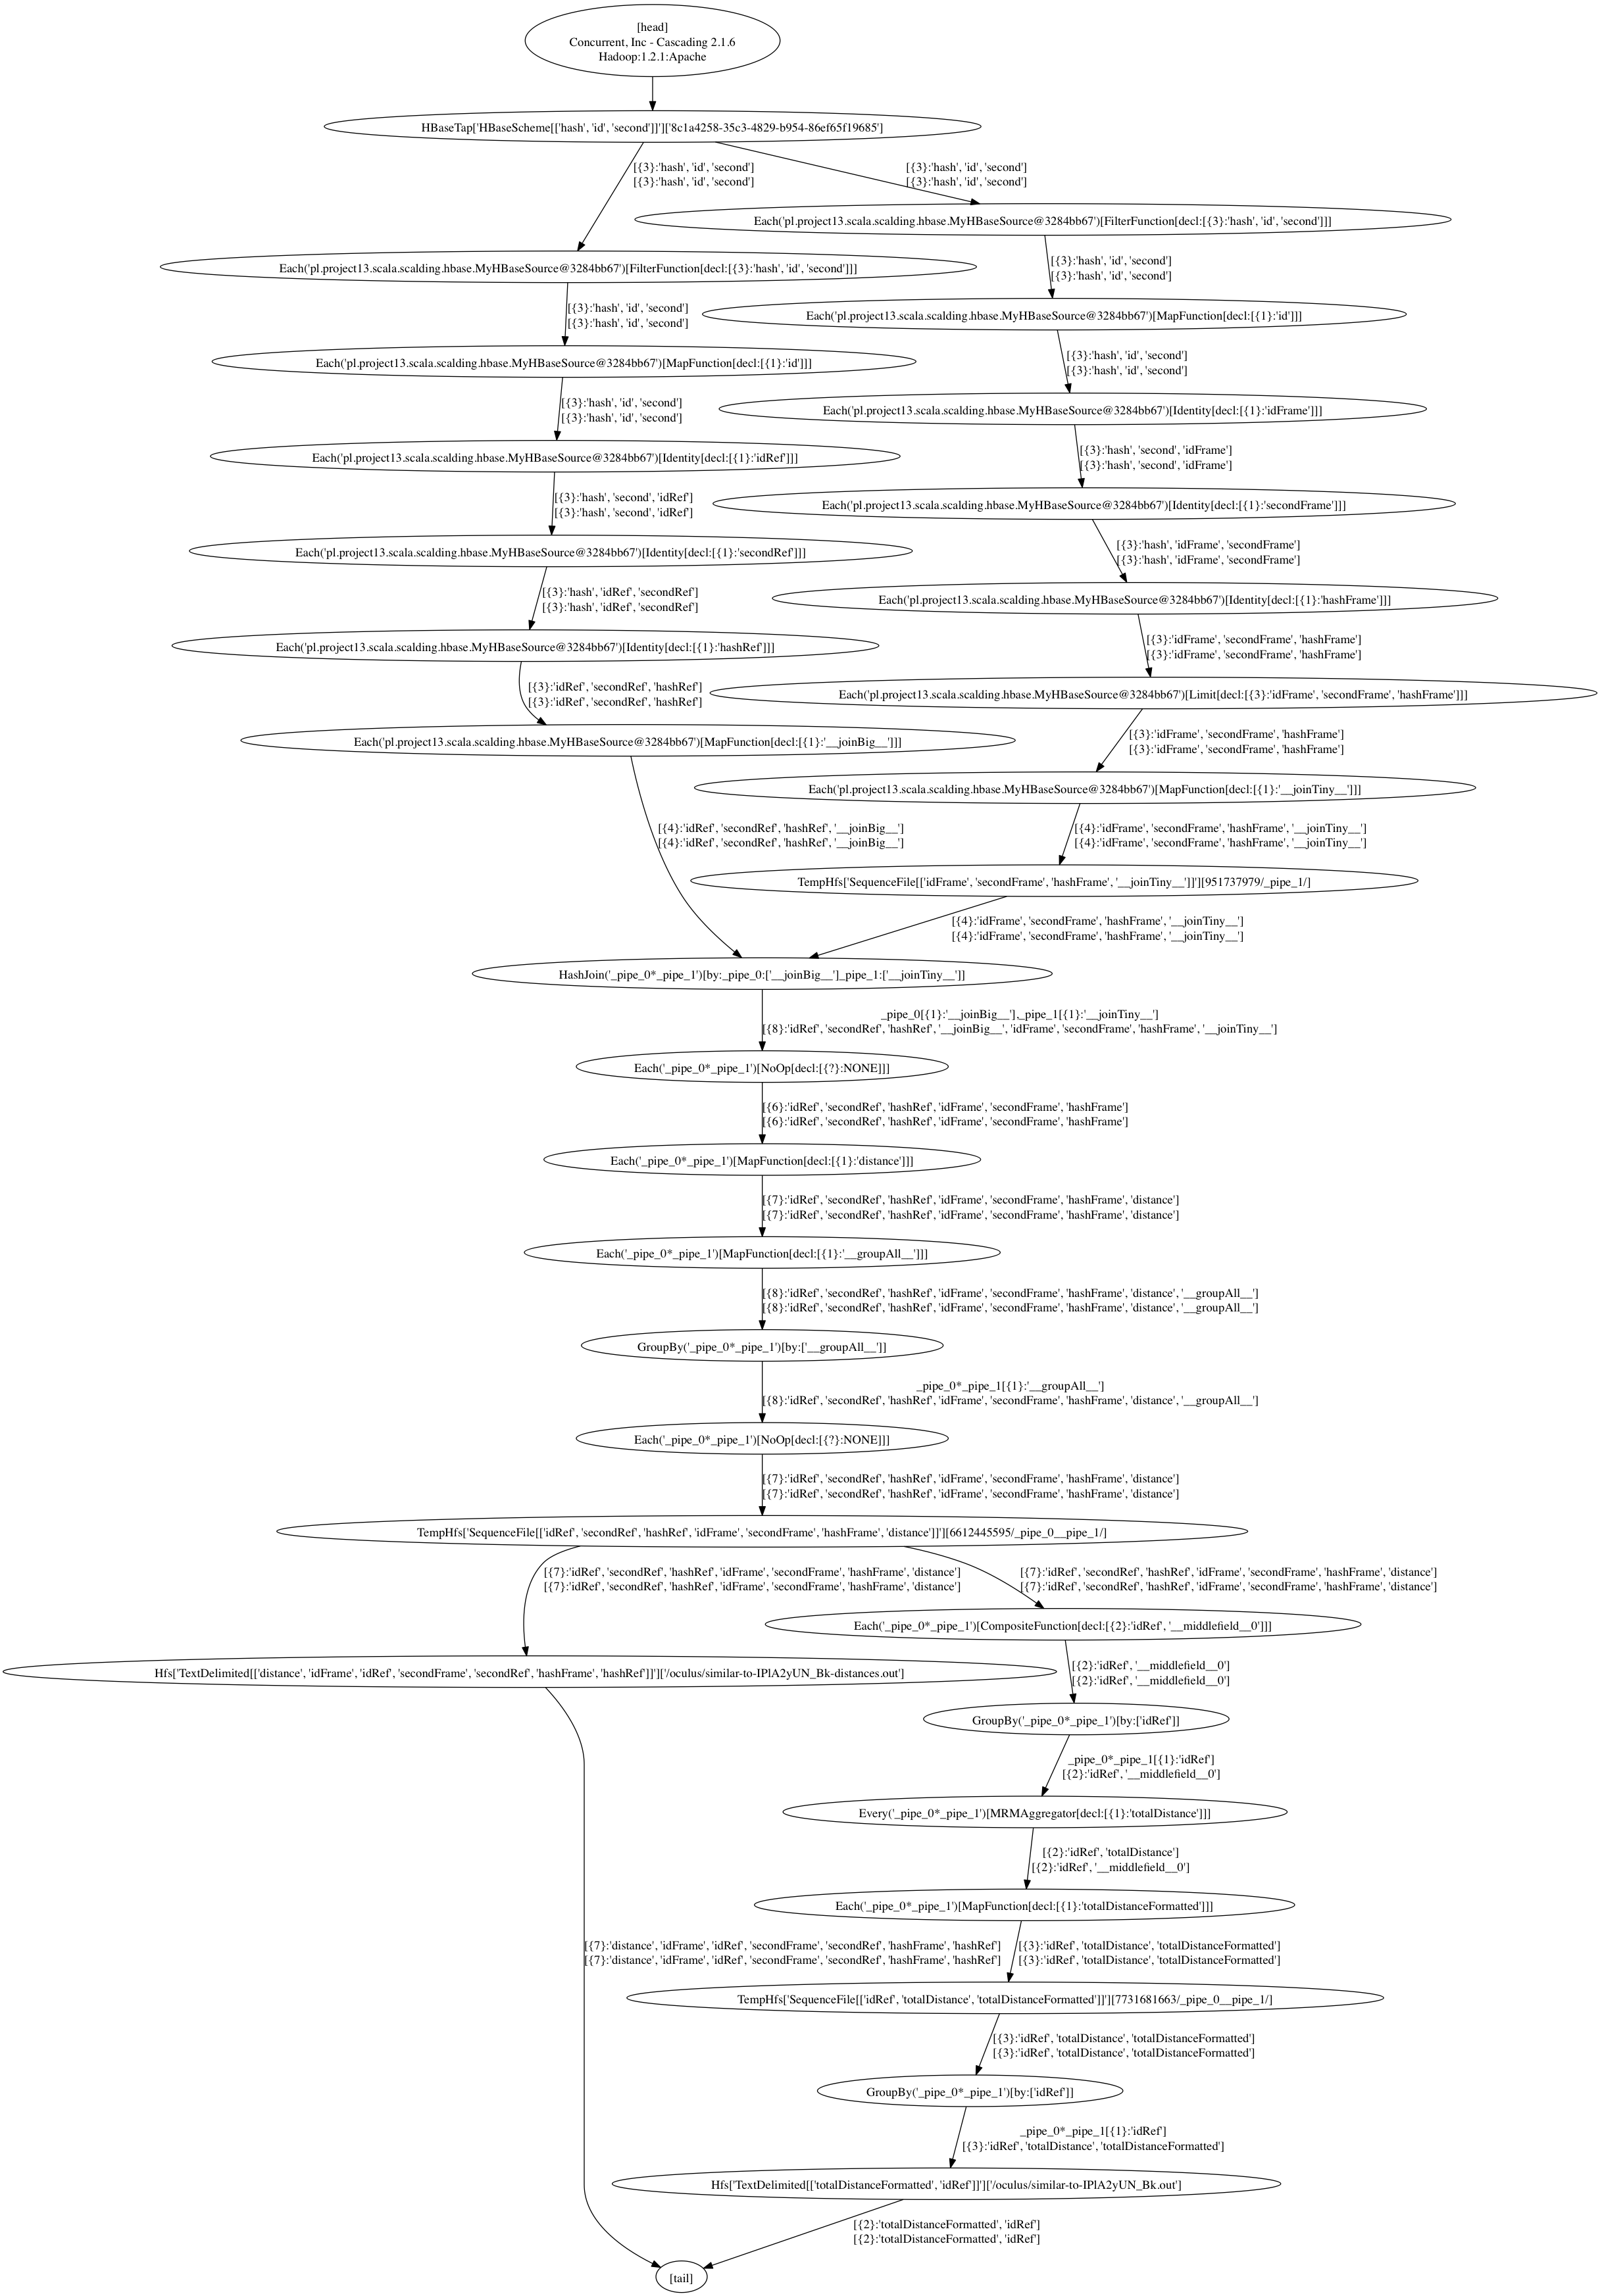
\includegraphics[width=0.9\textwidth]{img/FindSimilarMoviesJob_dot.png}
  \label{fig:find-similar-movies-most-complicated}
  \caption{This flow represents the most longest Pipeline preset in Oculus -- finding which movies are similar to the current one, ordered by ranking. It is constructed from 5 Map Reduce jobs.}
\end{figure}

Figure \ref{fig:find-similar-movies-most-complicated} represents the ''Find similar movies to the given one'' pipeline. Each circle represents an operation (such as emitting a tuple, grouping etc) and lines represent the data flowing through the Map Reduce jobs. It is also clearly visible that this pipeline consists of 5 map reduce jobs, where the 3rd job's input depends on jobs 1 and 2, and only after job 3 has completed jobs 4 and 5 can be executed (in parallel).

Sometimes though it is not easy to determine from this diagram alone how many actual MR Jobs a pipeline has emitted. For this reason we can instruct Cascading to print a DOT file containing the ''steps'', which for the algorithm represented in Listing \ref{lst:find-similar-movies-most-complicated-lst} Figure \ref{fig:find-similar-movies-most-complicated} would look like Figure \ref{fig:find-similar-movies-most-complicated-steps}.

\begin{lstlisting}[caption={Fragments of FindMostSimilarMoviesJob.dot}, label={lst:find-similar-movies-most-complicated-lst}]
digraph G {
1  [label = "Hfs['TextDelimited[[UNKNOWN] -> 
               ['refHash', 'frameHash', 'distance']]']['out']"];
2  [label = "Each('_pipe_0*_pipe_1')[NoOp[decl:[{?}:NONE]]]"];
3  [label = "GroupBy('_pipe_0*_pipe_1')[by:['__groupAll__']]"];
15 [label = "[tail]"];
# ...
    
4->3  [label = "[{4}:'refHash', 'frameHash', 'distance', '__groupAll__']
                [{4}:'refHash', 'frameHash', 'distance', '__groupAll__']"];
3->2  [label = "_pipe_0*_pipe_1[{1}:'__groupAll__']
                [{4}:'refHash', 'frameHash', 'distance', '__groupAll__']"];
1->15 [label = "[{3}:'refHash', 'frameHash', 'distance']
                [{3}:'refHash', 'frameHash', 'distance']"];
2->1  [label = "[{3}:'refHash', 'frameHash', 'distance']
                [{3}:'refHash', 'frameHash', 'distance']"];
# ...
}
\end{lstlisting}


\begin{figure}[ch!]
  \centering
  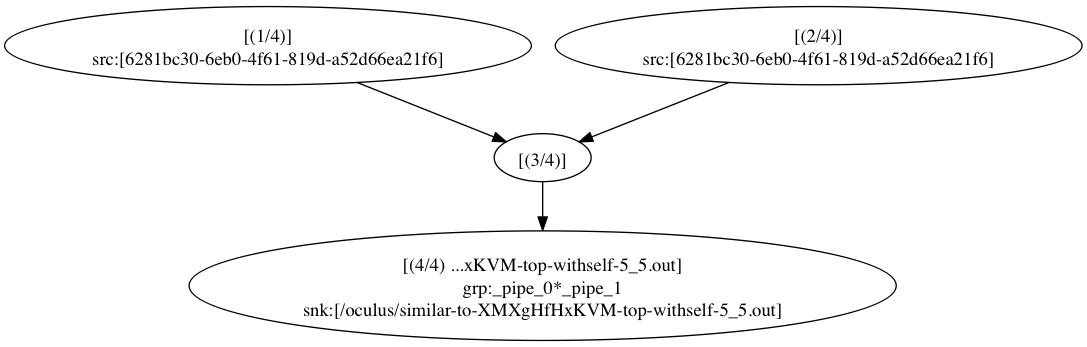
\includegraphics[width=0.9\textwidth]{img/FindSimilarMoviesV2Job-steps_dot.png}
  \label{fig:find-similar-movies-most-complicated-steps}
  \caption{A graph representation of the Map Reduce jobs that have to be run in order to complete the pipeline.}
\end{figure}
\todo{the steps DOT is wrong here}

The graph represented on Figure \ref{fig:find-similar-movies-most-complicated-steps} displays the same pipeline as Figure \ref{fig:find-similar-movies-most} but on a higher level -- displaying only the order and dependencies of each Map Reduce job. Step \verb|3/4| is easily identifiable as ''groupBy'' here, although from this graph we are unable to determine on what field we're grouping.

\todo{use I, not WE this is not a blog post...}

\todo{needs complete rewrite, slower with examples, show code of the task}






